
\section{Introduction}
The prevalence of positioning devices has drastically boosted 
the scale and spectrum of trajectory collection to an unprecedented level. 
Tremendous amounts of trajectories, in the form of sequenced spatial-temporal 
records, are continually generated from animal telemetry chips, 
vehicle GPSs and wearable devices. Data analysis on large-scale 
trajectories benefits a wide range of applications and services, 
including traffic planning~\cite{zheng2011urban}, animal analysis~\cite{li2010miningperiodic}, and social recommendations~\cite{bao2013survey}, to name just a few.

A crucial task of data analysis on top of trajectories is 
to discover co-moving objects. A \emph{co-movement} pattern~\cite{li2013managing,zheng2015survey} 
refers to a group of objects traveling together for a certain period of time 
and the group is normally determined by their spatial proximity. 
A pattern is prominent if the size of the group exceeds $M$ and the length of the duration exceeds $K$, where $M$ and $K$ are parameters specified by users. Rooted from such a basic definition 
and driven by different mining applications, there are a bunch of variants 
of co-movement patterns that have been developed with more advanced constraints.

Table~\ref{tbl:existing_co_patterns} summarizes several popular co-moving patterns 
with different constraints in the attributes of clustering in spatial proximity,
consecutiveness in temporal duration and computational complexity. 
In particular,  the \emph{flock}~\cite{gudmundsson2006flock} 
and the \emph{group}~\cite{wang2006grouppattern} patterns require 
all the objects in a group to be enclosed by a disk with radius $r$; 
whereas the \emph{convoy}~\cite{jeung2008convoy}, the \emph{swarm}~\cite{li2010swarm} 
and the \emph{platoon}~\cite{li2015platoon} patterns resort to density-based 
spatial clustering. 
In the temporal dimension, the \emph{flock}~\cite{gudmundsson2006flock} 
and the \emph{convoy}~\cite{jeung2008convoy} require all the timestamps 
of each detected spatial group to be consecutive, which is referred to as \emph{global consecutiveness}; 
whereas the \emph{swarm}~\cite{li2010swarm} does not impose any restriction. 
The \emph{group}~\cite{wang2006grouppattern} and the \emph{platoon}~\cite{li2015platoon} adopt a compromised manner by allowing
arbitrary gaps between the consecutive segments, which is called \emph{local consecutiveness}. 
They introduce a parameter $L$ to control the minimum length of each local consecutive segment.

\begin{figure}[h]
\centering
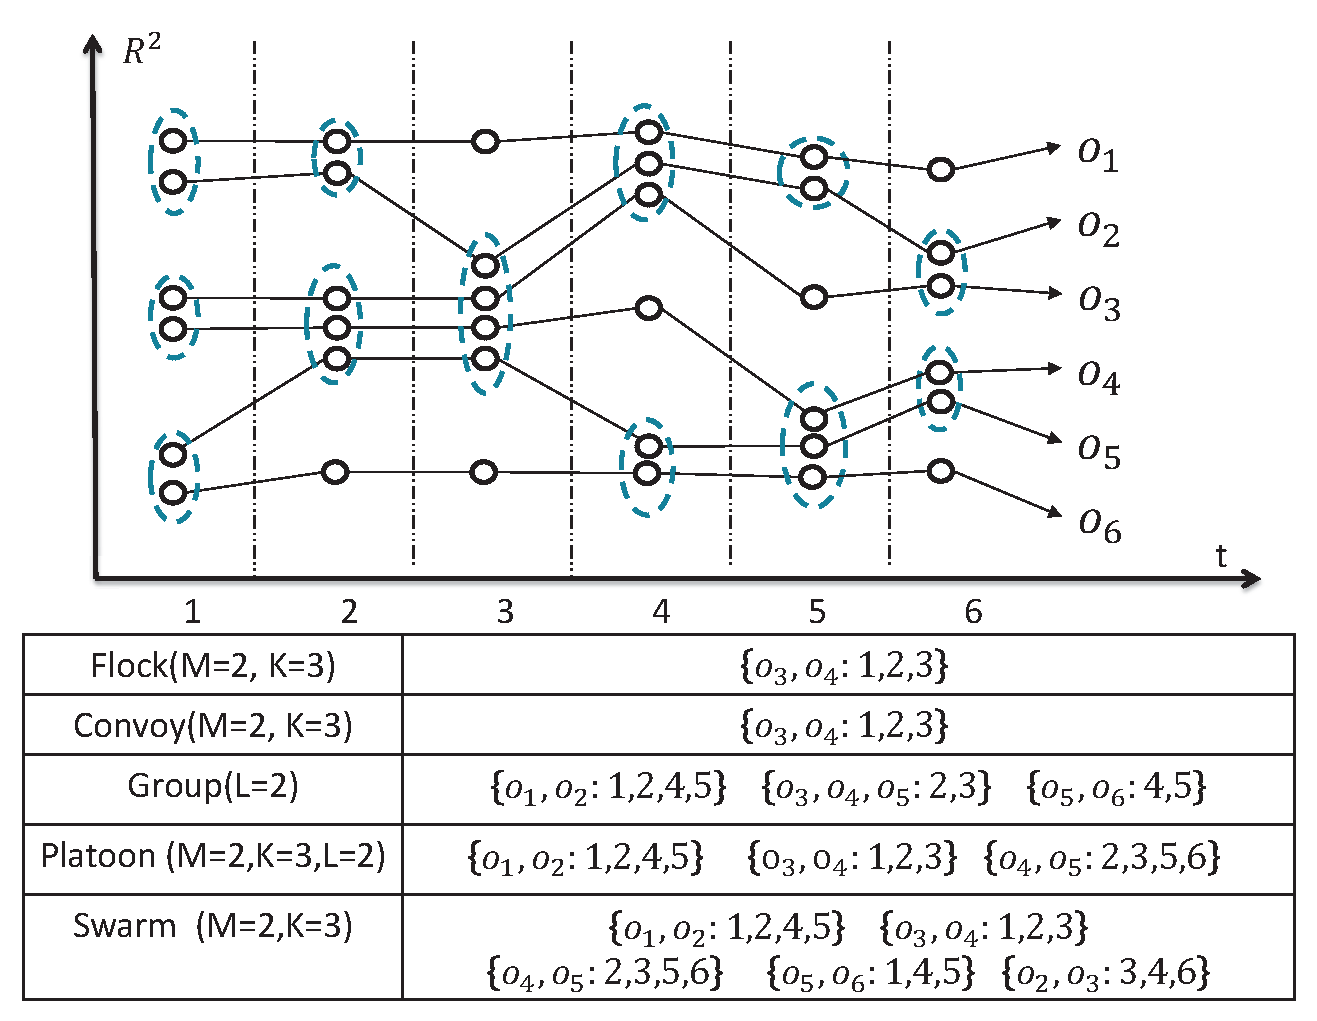
\includegraphics[width=0.45\textwidth]{related_work.eps}
\caption{Trajectories and co-movement patterns. The example consists of six trajectories across six snapshots. Objects in spatial clusters are enclosed by dotted circles. $M$ is the minimum cluster cardinality; $K$ denotes the minimum number of snapshots for the occurrence of a spatial cluster; and $L$ denotes the minimum length for local consecutiveness.}
\label{fig:related_work}
\end{figure}

Figure~\ref{fig:related_work} is an example to demonstrate the concepts of various co-movement patterns. The trajectory database consists of six moving objects and the temporal dimension is discretized into six snapshots. In each snapshot, we treat the clustering method as a black-box and assume that they generate the same clusters. Objects in proximity are grouped in the dotted circles. As aforementioned, there are three parameters to determine the co-movement patterns and the default settings in this example are $M=2$, $K=3$ and $L=2$. Both the \emph{flock} and the \emph{convoy} require the spatial clusters to last for at least $K$ consecutive  timestamps. Hence,$\langle o_3,o_4:1,2,3 \rangle$ and $\langle o_5,o_6:3,4,5 \rangle$  remains the only two candidates matching the patterns. The \textit{swarm} relaxes the pattern matching by discarding the temporal consecutiveness constraint. Thus, it generates many more candidates than the \textit{flock} and the \textit{convoy}. The \textit{group} and the \textit{platoon} add another constraint on local consecutiveness to retain meaningful patterns. For instance, $\langle o_1,o_2:1,2,4,5 \rangle$ is a pattern matching local consecutiveness because timestamps $(1,2)$ and $(4,5)$ are two segments with length no smaller than $L=2$. The difference between the \textit{group} and the \textit{platoon} is that the \textit{platoon} has an additional parameter $K$ to specify the minimum number of snapshots for the spatial clusters. This explains why $\langle o_3,o_4,o_5:2,3 \rangle$ is a  \textit{group} pattern but not a \textit{platoon} pattern.

As can be seen, there are various co-movement patterns requested by different applications and it is cumbersome to design a tailored solution for each type. In addition, despite the generality of the \emph{platoon} (i.e., it can be reduced to other types of patterns via proper parameter settings), it suffers from the so-called \emph{loose-connection} anomaly. We use two objects $o_1$ and $o_2$ in Figure~\ref{fig:platoon_weakpoint} as an example to illustrate the scenario. These two objects form a \emph{platoon} pattern in timestamps $(1,2,3,102,103,104)$. However, the two consecutive segments are $98$ timestamps apart, resulting in a false positive co-movement pattern. In reality, such an anomaly may be caused  by the periodic movements of unrelated objects, such as vehicles stopping at the same petrol station or animals pausing at the same water source. 
Unfortunately, none of the existing patterns have directly addressed this anomaly.

\begin{figure}[h]
\center
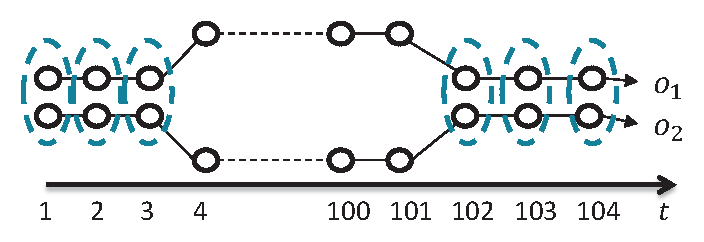
\includegraphics[width=0.3\textwidth]{platoon_weakpoint.eps}
\caption{\emph{Loose-connection} anomaly. Even though $\langle o_1, o_2: 1,2,3,102,103,104 \rangle$ is considered as a valid \emph{platoon} pattern, it is highly probable that these two objects are not related as the two consecutive segments  are 98 timestamps apart. 
}
\label{fig:platoon_weakpoint}
\end{figure}

\begin{table} \scriptsize
\centering
\begin{tabular}{|l|l|c|l|}
\hline 
\textbf{Pattern} & {\tiny \textbf{Proximity}} & {\tiny \textbf{Consecutiveness}} & {\tiny \textbf{Time Complexity}}\\ 
\hline 
flock~\cite{gudmundsson2004flock} & disk-based &  global & {\tiny $O(|\mathbb{O}||\mathbb{T}|\log(|\mathbb{O}|))$} \\ 
\hline 
convoy~\cite{jeung2008convoy} & density-based &   global & {\tiny $O(|\mathbb{O}|^2+|\mathbb{O}||\mathbb{T}|)$}\\ 
\hline 
swarm~\cite{li2010swarm} & density-based  & - & {\tiny $O(2^{|\mathbb{O}|}|\mathbb{O}||\mathbb{T}|)$}  \\ 
\hline 
group~\cite{wang2006grouppattern} & disk-based &  local & {\tiny $O(|\mathbb{O}|^2|\mathbb{T}|)$}\\ 
\hline 
platoon~\cite{li2015platoon} & density-based &  local & {\tiny $O(2^{|\mathbb{O}|}|\mathbb{O}||\mathbb{T}|)$}\\ 
\hline 
\end{tabular} 
\caption{Constraints and complexities of co-movement patterns. The time complexity indicates the performance wrt.
$|\mathbb{O}|$, $|\mathbb{T}|$ in the worst case, where $|\mathbb{O}|$ is the number of objects, and $|\mathbb{T}|$ is the number of discretized timestamps.}
\label{tbl:existing_co_patterns}
\end{table}
The other issue with existing methods is that they are built on top of centralized indexes which may not be scalable. Table~\ref{tbl:existing_co_patterns} shows their theoretical complexities in the worst cases and the largest real dataset ever evaluated in previous studies is up to million-scale points collected from hundreds of moving objects. In practice, the dataset is of much higher scale and the scalability of existing methods is left unknown. Thus, we conduct an experimental evaluation with $4000$ objects moving for $2500$ timestamps to examine the scalability. Results in Figure~\ref{fig:related_work_scalability} show that their performances degrade dramatically as the dataset scales up. For instance, the detection time of \emph{group} drops twenty times as the number of objects grows from \emph{1k} to \emph{4k}. Similarly,
the performance of \emph{swarm} drops over fifteen times as the number of snapshots grows from \emph{1k} to \emph{2.5k}.
These observations imply that existing methods are not scalable to support large-scale trajectory databases. 

\begin{figure}[h]
	\vspace{-3mm}
    \centering
    \begin{subfigure}[b]{0.23\textwidth}
            \centering
            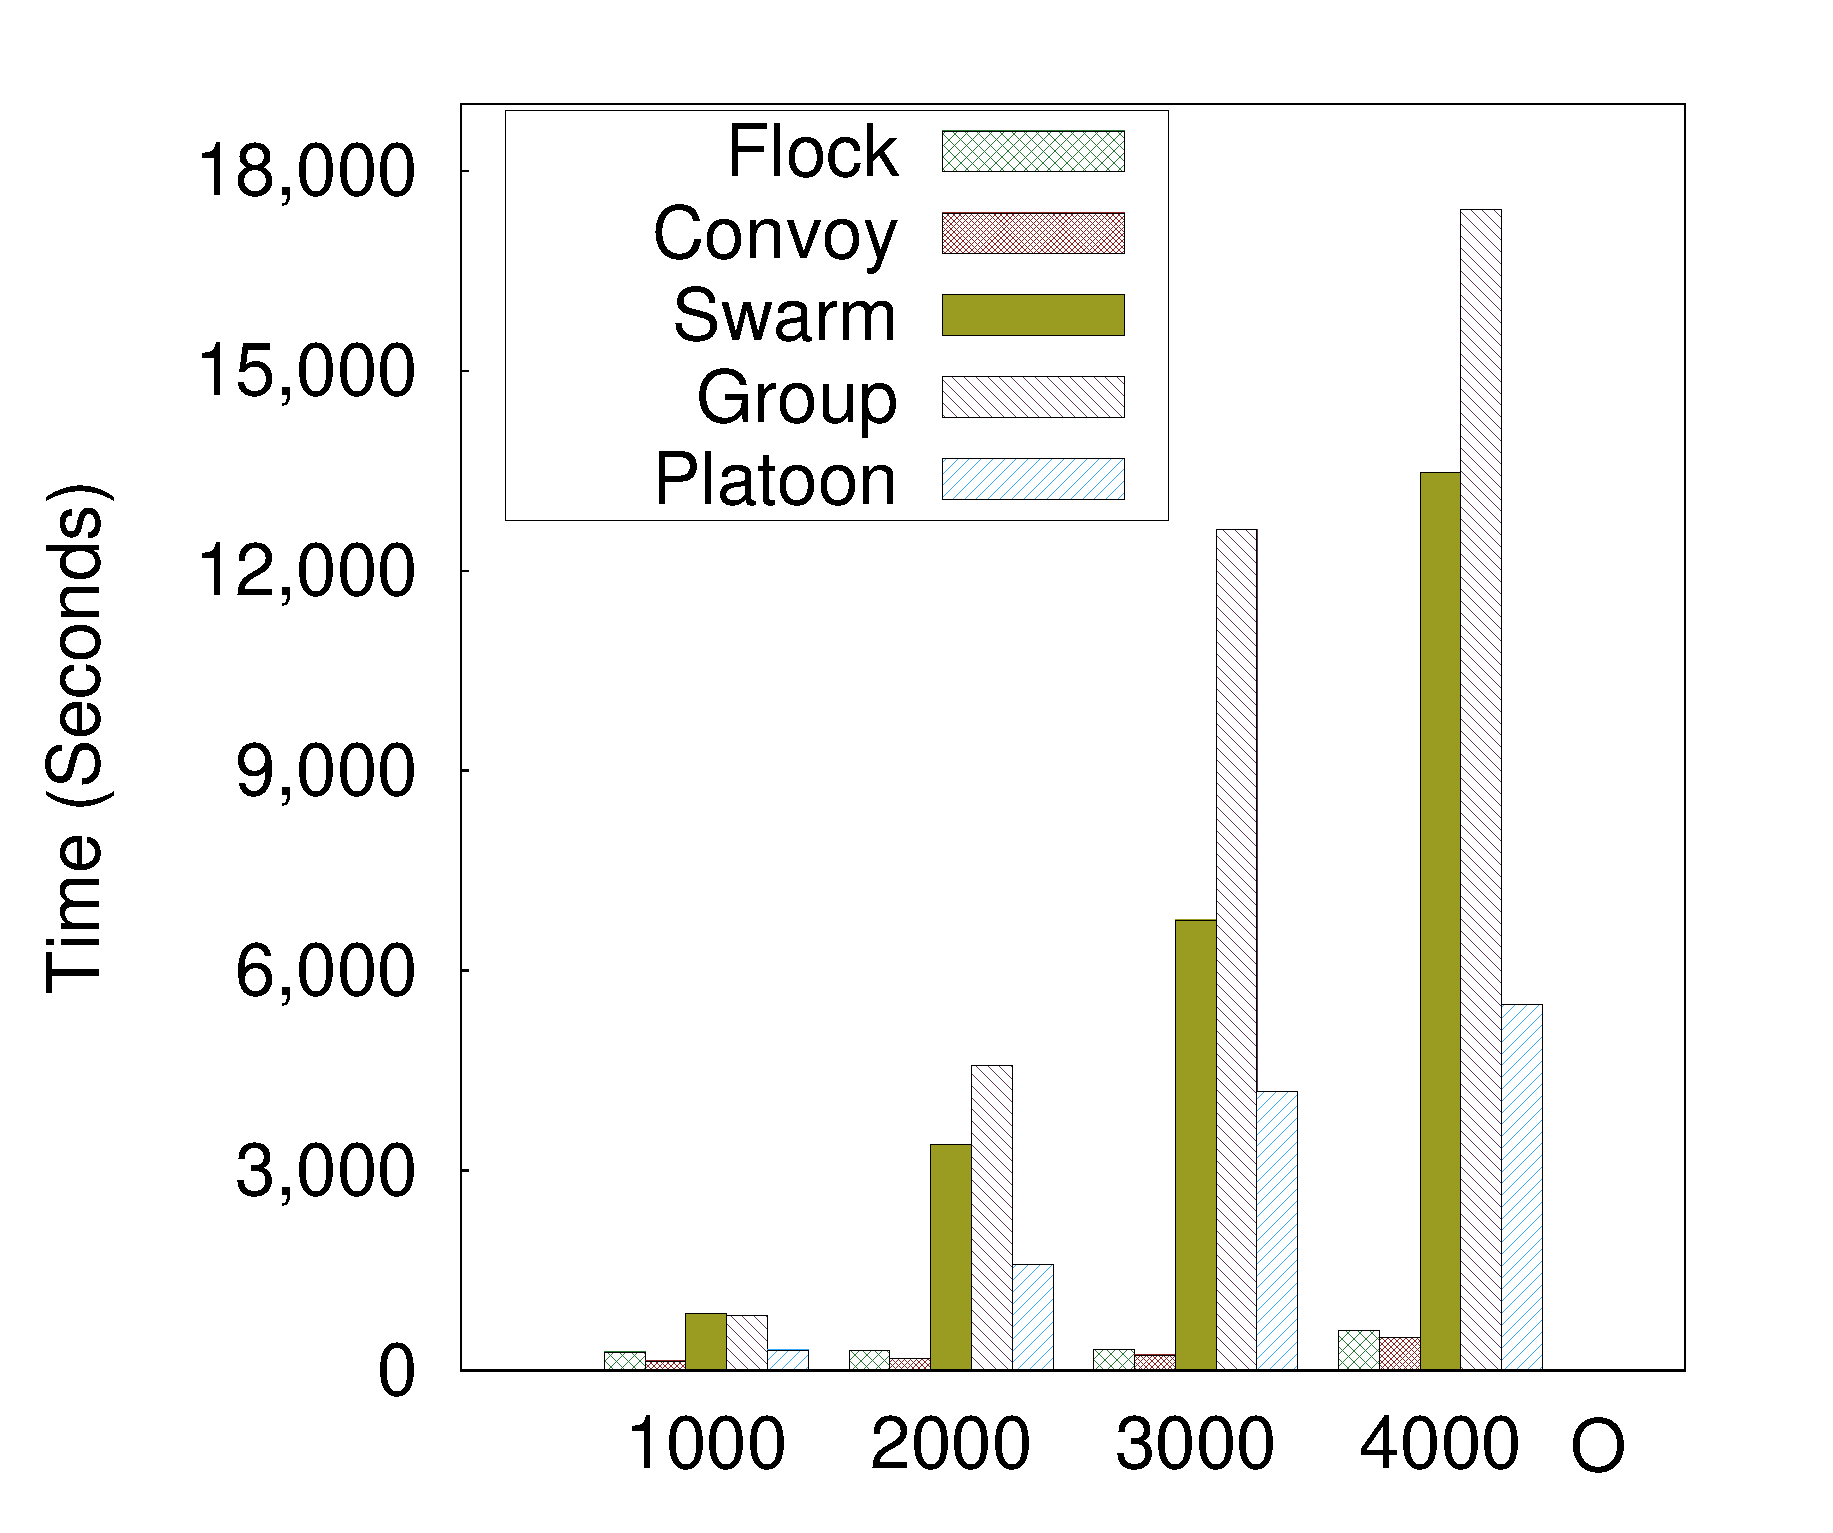
\includegraphics[width=\textwidth]{rw_perf_O.eps}
		\subcaption{\small Varying No. of objects} 
    \label{fig:fig1}
    \end{subfigure}
    \begin{subfigure}[b]{0.23\textwidth}
            \centering
            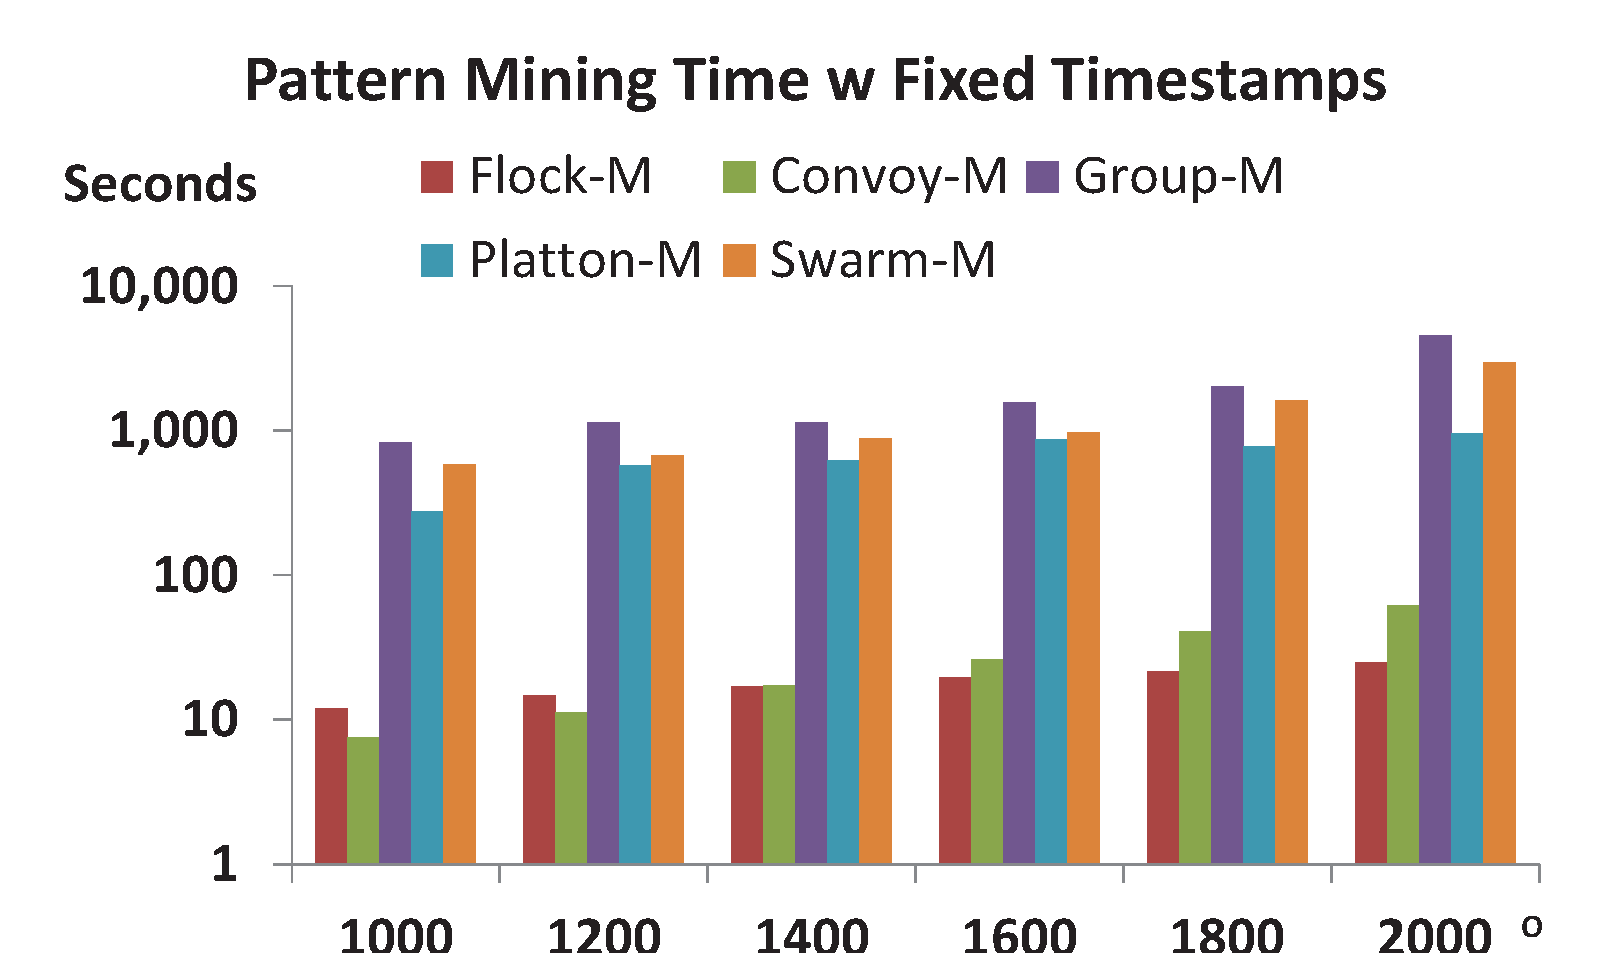
\includegraphics[width=\textwidth]{rw_perf_T.eps}
         \subcaption{\small Varying No. of timestamps}
    \label{fig:fig2}
    \end{subfigure}
    \vspace{-2mm}
    \caption{Performance measures on existing co-movement patterns. A sampled GeoLife dataset
    is used with up two 2.4 million data points. Default parameters are $M=15$, $K=180$, $L=30$.}
    \label{fig:related_work_scalability}
\end{figure}

Therefore, our primary contributions in this paper are to close these two gaps. 
First, we propose the \emph{general co-movement pattern} (GCMP) which models
various co-moment patterns in a unified way and can avoid 
the \emph{loose-connection} anomaly. In GCMP, we introduce a new gap parameter $G$ to pose a constraint on the temporal gap between two consecutive segments. By setting a feasible $G$, the loose-connection anomaly can be effectively controlled. In addition, our GCMP is both general and expressive. It can be reduced to any of the previous patterns by customizing its parameters.

Second, we investigate deploying our GCMP detector on MapReduce platforms (such as Hadoop and Spark) to tackle the scalability issue. Our technical contributions are three-fold. First, we design a baseline solution by replicating the snapshots in multiple data chunks to support effective parallel mining. Second, we devise a novel \emph{Star Partitioning and ApRiori Enumerator} (SPARE) framework to resolve limitations of the baseline. SPARE achieves workload balance by partitioning objects into fine granular stars.  For each star partition, an Apriori Enumerator is adopted to mine the co-movement patterns. Third, we leverage the \emph{temporal monotonicity} property of GCMP 
to design several optimization techniques including \emph{sequence simplification}, \emph{monotonicity pruning} and \emph{forward closure check} to further reduce the number of candidates enumerated in SPARE.

We conduct a set of extensive experiments on three large-scaled real datasets with hundreds of millions of
temporal points. 
The results show that both our parallel schemes efficiently support GCMP mining in large datasets.
In particular, with over 170 million trajectory points,
SPARE achieves upto 112 times speedup using 162 cores as compared to the state-of-the-art centralized schemes.
Moreover, SPARE further achieves upto 14 times efficiency
as compared to the baseline algorithm with almost linear scalability.

The rest of our paper is organized as follows: Section~\ref{sec:related_works} summarizes the relevant literature on 
trajectory pattern mining. Section~\ref{sec:definition} defines the problem of general co-movement pattern mining. Section~\ref{sec:trm} provides a baseline solution. An advanced solution named
\emph{Star Partitioning and ApRiori Enumerator} (SPARE) is presented in Section~\ref{sec:spm}. Section~\ref{sec:exp} conducts extensive experiments to verify the efficiency of our solutions. Finally, Section~\ref{sec:concl} concludes the paper.
